\section{Introduction} 
\subsection{Problem Statement:}
%\vspace{-10mm}
\begin{wrapfigure}[14]{r}{60mm}
  \begin{center}
    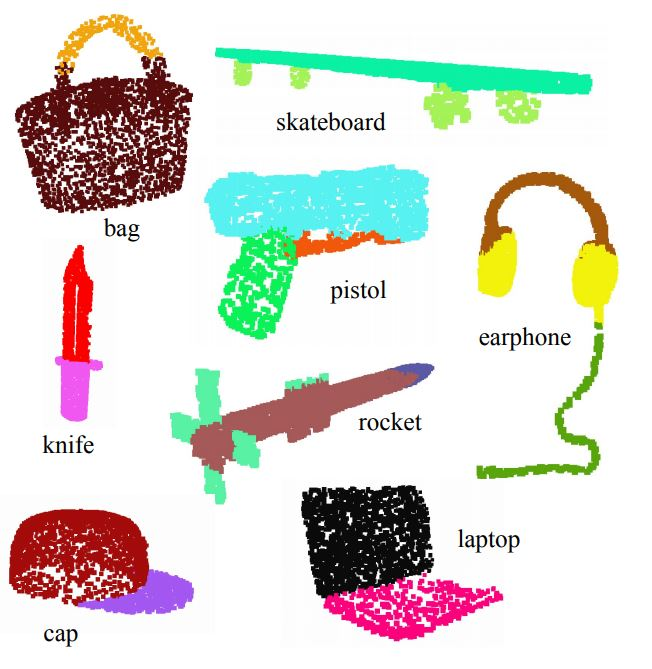
\includegraphics[width=0.3\textwidth]{fig/ex.JPG}
  \end{center} 
  \caption*{Example Models (color here are added for visualization only).}
\end{wrapfigure}

In this project we are trying to classify 3D point cloud. The data set is sets of \emph{models}. Each model is comprised of a set of $n$ data points. A data points is a tuple of 3D coordinates ($x,y,z$) of the point in the space. Figure on the left shows few examples of the data set we have. Each model is associated with a label (for training) shown under the model. 

The data set consists (ModelNet40 \citep{wu20153d}) of 9840 models for training and 2468 models for testing. Our task is to create a CNN model that can train such data set and achieve good accuracy within the test models. 


\subsection{Challenges:}
At first glance the classification looks similar to classifying images which has been investigated thoroughly in the past couple of years. However, we a careful look at the problem and the type of input we have, we can realize the following set of challenges that will influence our model
\paragraph{Irregularity:}
While standard deep neural network models take as input data with regular structure (images of a fixed sizes), point clouds are irregular. This means we have no expectation of the input size (the number of points per models). The reason behind this is that these models either come from scan operations or hand-crafted which can not be constrained to give models of fixed size.

\paragraph{Unordered:} Point positions are continuously distributed in the space and any permutation of their ordering does not change the spatial distribution. The model is read from a file which could store the point in a certain order that is different than other similar models. Thus, associating the feature with the point order could be misleading.
\paragraph{Invariance:} The learned features should be invariant to translation and rotation. Our model should be able to accurately similar models even if they are rotated or shifted. Similar case exists in image where a certain feature could be located anywhere in the image. However, with point cloud in 3D space the problem is augmented as there is a third degree of freedom for translation and rotation. 



\subsection{Previous Work:}
Previous work on point cloud classification using CNN has three main directions:
\paragraph{View-based Methods:}
These methods represents a single model as a collection of 2D views to which standard CNNs used in image classification can be employed directly. View-based appraoches are good match for applications where the input comes from 3D sensor and represented as a range image in which case a single view can be used~\citep{wei2016dense}. 

\paragraph{Volumetric Methods:}
Voxelization is another straightforward way to convert irregular data set to a regular 3D grid over which standard CNN can be applied~\citep{maturana2015voxnet}. Voxelization produces a sparsely-occupied grids and induce quantization artifacts. Cleverer space partition like $k$-d tree can be used to mitigate these problem~\citep{klokov2017escape}.
\paragraph{Direction Methods}